\section{Loops}
\label{sec:loops}
\begin{frame}<beamer>
    \frametitle{Outline}
    \tableofcontents[currentsection]
\end{frame}

\begin{frame}[fragile]{An opening example}
\begin{itemize}
	\item {Calculate $S=\sum_{x=1}^5\frac{1}{x^2}$}
	\item {Based on what we learn, we do it in following way}
\end{itemize}
\vspace{-0.15in}
\begin{columns}
\begin{column}{0.5\linewidth}
\begin{lstlisting}
int main()
{
   int x = 1;
   double S = 0;
   S += 1.0/(x*x);
   x += 1;
   S += 1.0/(x*x);
   x += 1;
   S += 1.0/(x*x);
   x += 1;
   S += 1.0/(x*x);
   x += 1;
   S += 1.0/(x*x);
   printf("S = %lf\n", S);
   return 0;
}
\end{lstlisting}
\end{column}
\begin{column}{0.45\linewidth}
\begin{itemize}
	\item {It is okay when the number of terms is small}
	\item {How about 1000 terms ...}
	\item {Share the story}
\end{itemize}
\end{column}
\end{columns}

\end{frame}


\begin{frame}[fragile]{Motivation of loops}
\begin{itemize}
	\item {In the above example}
	\item {Following statement repeated for 5 times, only x changes each time}
\end{itemize}
\vspace{-0.15in}
\begin{lstlisting}
   x += 1;
   S += 1.0/(x*x);
\end{lstlisting}
\vspace{-0.1in}
\begin{itemize}
	\item {We can put it inside a loop}
	\item {Tell the loop that how many times we want to repeat}
\end{itemize}
\vspace{-0.05in}
\begin{lstlisting}
x = 0;
while(x <= 4)
{
   x += 1;
   S += 1.0/(x*x);
}
\end{lstlisting}
\end{frame}

\begin{frame}[fragile]{Loops}
\vspace{-0.1in}
\begin{itemize}
   \item {To repeat statements as long as a certain condition is \textcolor{red}{true} (non-zero)}
   \item {C offers 3 different loops}
   \item {We can replace one with another}
   \item {Different loop offers different convenience}
\end{itemize}
\vspace{-0.1in}
	\begin{lstlisting}[numbers=none]
while(condition)
   statement;
\end{lstlisting}
\vspace{-0.1in}
	\begin{lstlisting}[numbers=none]
do
    statement;
while(condition);
\end{lstlisting}
\vspace{-0.1in}
	\begin{lstlisting}[numbers=none]
for(initialization; condition; statement)
    statement;
\end{lstlisting}
	For multiple statements again, use \textcolor{red}{braces}.
\end{frame}

\subsection{while loop}
\label{sec:while}
\begin{frame}<beamer>
    \frametitle{Outline}
    \tableofcontents[currentsection,currentsubsection]
\end{frame}

\begin{frame}[fragile]{while loop control (1)}
\begin{itemize}
	\item {The execution checks if the condition is still non-zero}
	\item {If it is, execute the statement(s)}
	\item {Otherwise, gets out from the loop}
\end{itemize}
\begin{figure}
	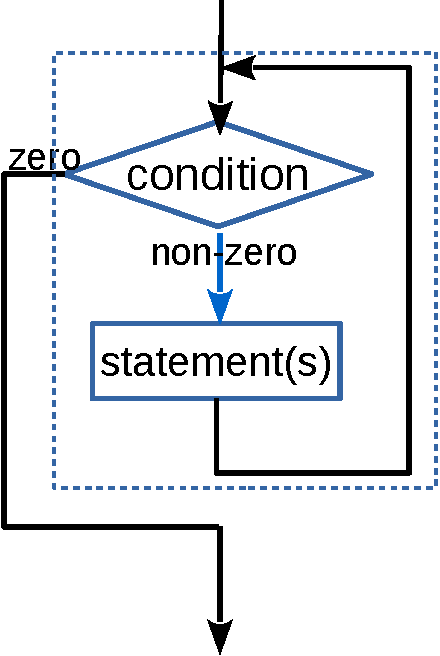
\includegraphics[width=0.25\linewidth]{figs/while.pdf}
\end{figure}
\end{frame}

\begin{frame}[fragile]{while loop control (2)}
\begin{itemize}
	\item {The execution of checks if the condition is still non-zero}
	\item {If it is, execute the statement(s)}
	\item {Otherwise, gets out from the loop}
\end{itemize}
	\begin{lstlisting}
int i = 2;
while (i > 0)
   --i;
printf("done\n");
\end{lstlisting}
\vspace{-0.15in}
\begin{enumerate}[<+(1)->]
	\item Check (i $>$ 0) $\rightarrow$ \textbf{true} $\rightarrow$ go to line 3
	\item Decrement i $\rightarrow$ i now is \textbf{1}, go back to line 2
	\item Check (i $>$ 0) $\rightarrow$ \textbf{true} $\rightarrow$ go to line 3
	\item Decrement i $\rightarrow$ i now is \textbf{0}, go back to line 2
	\item Check (i $>$ 0) $\rightarrow$ \textbf{false} $\rightarrow$ go to line 4
	\item Print \textbf{done}
\end{enumerate}
\end{frame}

\begin{frame}[fragile]{Check Prime Number (1)}
\begin{itemize}
	\item {Check whether an integer number if a prime number}
	\item {Prime number: number that is only dividable by 1 and itself}
	\item {81 is not a prime number; 173 is prime number}
	\item {Any idea to solve this problem??}
\end{itemize}

\begin{center}
	\Large{5 minutes to think about this problem ...}
\end{center}
\end{frame}

\begin{frame}[fragile]{Check Prime Number (2)}
\vspace{-0.2in}
\begin{enumerate}
	\item {Start from 2 to N}
	\item {Check whether N is dividable by any number in this range}
\end{enumerate}
	\begin{lstlisting}[linewidth=0.7\linewidth]
int i = 2, N = 177;
int _PRIME_ = 1;
while(i < N)
{
    if(N%i == 0)
    {
        _PRIME_ = 0;
    }
}
if(_PRIME_)
   printf("%d is a prime number\n", N);
else
   printf("%d is not a prime number\n", N);
\end{lstlisting}
\vspace{-0.1in}
\begin{itemize}
	\item {Do we \textcolor{red}{miss} anything?}
\end{itemize}
\end{frame}

\begin{frame}[fragile]{Check Prime Number (3)}
\begin{enumerate}
	\item {Start from 2 to N}
	\item {Check whether N is dividable by any number in this range}
\end{enumerate}
\begin{center}

	\begin{lstlisting}[linewidth=0.7\linewidth]
int i = 2, N = 177;
int _PRIME_ = 1;
while(i < N)
{
    if(N%i == 0)
    {
        _PRIME_ = 0;
    }
    i++;
}
if(_PRIME_)
   printf("%d is a prime number\n", N);
else
   printf("%d is not a prime number\n", N);
\end{lstlisting}

\end{center}
\end{frame}

\begin{frame}[fragile]{Check Prime Number (4)}
\vspace{-0.1in}
\begin{enumerate}
	\item {In the above example, we no need to all the numbers in [2$\cdots$N-1]}
	\item {N is not dividable by numbers after $\lceil\sqrt{N}\rceil$}
\end{enumerate}
	\begin{lstlisting}[basicstyle=\scriptsize,linewidth=0.7\linewidth]
#include <stdio.h>
#include <math.h>
int main()
{
  int i = 2, N = 177;
  int _PRIME_ = 1, bnd = (int)ceil(sqrt(N));
  while(i <= bnd)
  {
    if(N%i == 0)
    {
        _PRIME_ = 0;
    }
    i++;
  }
  if(_PRIME_)
    printf("%d is a prime number\n", N);
  else
   printf("%d is not a prime number\n", N);
  return 0;
}
\end{lstlisting}
\end{frame}

\subsection{do-while loop}
\begin{frame}<beamer>
    \frametitle{Outline}
    \tableofcontents[currentsection,currentsubsection]
\end{frame}

\begin{frame}[fragile]{do...while (1)}
\begin{itemize}
	\item {\textcolor{blue}{do}...\textcolor{blue}{while} executes the statement(s) first}
	\item {Checks the condition after each run}
\end{itemize}	
\begin{columns}
\begin{column}{0.42\linewidth}
\begin{lstlisting}
int i = 3;
do
{   
   --i;
   printf("i=%d\n", i);
}while (i > 1);
\end{lstlisting}
\end{column}
\begin{column}{0.1\linewidth}
\end{column}
\begin{column}{0.42\linewidth}
\begin{lstlisting}
int i = 3;
while(i > 1)
{
   --i;
   printf("i=%d\n", i);
}
\end{lstlisting}
\end{column}
\end{columns}
\begin{itemize}
	\item {What is the output??}
\end{itemize}
\end{frame}

\begin{frame}[fragile]{do...while (2)}
\begin{itemize}
	\item {\textcolor{blue}{do}...\textcolor{blue}{while} executes the statement(s) first}
	\item {Checks the condition after each run}
\end{itemize}	
\begin{columns}
\begin{column}{0.4\linewidth}
\begin{lstlisting}
i=2
i=1
\end{lstlisting}
\end{column}
\begin{column}{0.1\linewidth}
\end{column}
\begin{column}{0.4\linewidth}
\begin{lstlisting}
i=2
i=1
\end{lstlisting}
\end{column}
\end{columns}
\begin{itemize}
	\item {What is the output??}
\end{itemize}
\end{frame}

\begin{frame}[fragile]{do...while (3)}
\begin{itemize}
	\item {\textcolor{blue}{do}...\textcolor{blue}{while} executes the statement(s) first}
	\item {Checks the condition after each run}
\end{itemize}	
\begin{figure}
	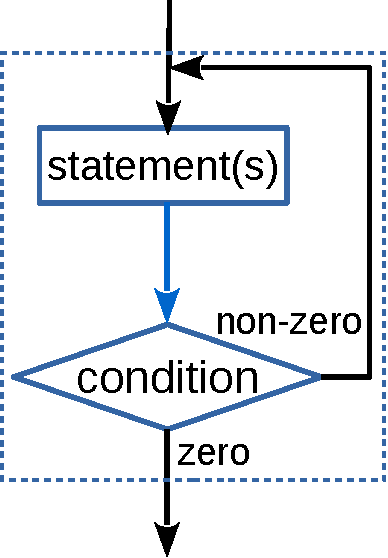
\includegraphics[width=0.30\linewidth]{figs/dowhile.pdf}
\end{figure}
\end{frame}


\begin{frame}[fragile]{Example 1 (1)}
\begin{itemize}
	\item {Calculate $x=\sqrt{a}$}
	\item {$x_{n+1}=\frac{1}{2}(x_n+\frac{a}{x_n})$}
	\item {Loop until error less than $10^{-5}$ in consecutive iterations}
	\item {Hints: $x_1$ is an arbitrary positive value}
\end{itemize}

\begin{center}
	\Large{3 minutes to think about this problem ...}
\end{center}

\end{frame}

\begin{frame}[fragile]{Example 1 (2)}
\begin{itemize}
	\item {Calculate $x=\sqrt{a}$}
	\item {$x_{n+1}=\frac{1}{2}(x_n+\frac{a}{x_n})$}
	\item {Loop until error less than $10^{-5}$ in consecutive iterations}
	\item {Hints: $x_1$ is an arbitrary positive value}
\end{itemize}

\begin{enumerate}
	\item {We need a loop (\textcolor{blue}{while}? \textcolor{blue}{do}-\textcolor{blue}{while} or \textcolor{blue}{for}?)}
	\item {We need to keep two results from consecutive iterations}
	\item {Anything else??}
	\item {Let's do it!}
\end{enumerate}

\end{frame}

\begin{frame}[fragile]{Example 1 (3)}
\begin{itemize}
	\item {Calculate $x=\sqrt{a}$}
	\item {$x_{n+1}=\frac{1}{2}(x_n+\frac{a}{x_n})$}
	\item {Loop until error less than $10^{-5}$ in consecutive iterations}
	\item {Hints: $x_1$ is an arbitrary positive value}
\end{itemize}
\begin{lstlisting}
  float a = 5, x0 = 3.1, xn = 0, err = 0;
  do
  {
     xn  = 0.5*(xn+a/xn);
     err = abs(xn - x0);
  }while(err >= 0.00001)
  printf("sqrt(a)=%f\n", xn);
\end{lstlisting}
\begin{itemize}
	\item {Anything wrong??}
\end{itemize}
\end{frame}

\begin{frame}[fragile]{Example 1 (4)}
\begin{itemize}
	\item {Calculate $x=\sqrt{a}$}
	\item {$x_{n+1}=\frac{1}{2}(x_n+\frac{a}{x_n})$}
	\item {Loop until error less than $10^{-5}$ in consecutive iterations}
	\item {Hints: $x_1$ is an arbitrary positive value}
\end{itemize}
\begin{lstlisting}
  float a = 5, xk = 0, xn =  3.1, err = 0;
  int i = 0;
  do
  {
     xk  = xn;
     xn  = 0.5*(xk+a/xk);
     //printf("%f\t%f\t%f\n", xk, xn, err);
     err = fabs(xn - xk);
     i++;
  }while(err >= 0.00001);
  printf("iters = %d, sqrt(a)=%f\n",  i, xn);
\end{lstlisting}
\begin{itemize}
	\item {Use ``\textcolor{red}{fabs}(.)'' instead of ``\textcolor{red}{abs}(.)''}
\end{itemize}
\end{frame}

\subsection{for loop}
\begin{frame}<beamer>
    \frametitle{Outline}
    \tableofcontents[currentsection,currentsubsection]
\end{frame}


\begin{frame}[fragile]{for loop (1)}
	The For-Loop is comfortable for iterating. It takes three arguments.
	\begin{itemize}
		\item {Initialization (i=0;)}
		\item {Condition ($i<5$;)}
		\item {Iteration statement (i+=1)}
	\end{itemize}
	\bigskip
\begin{figure}
	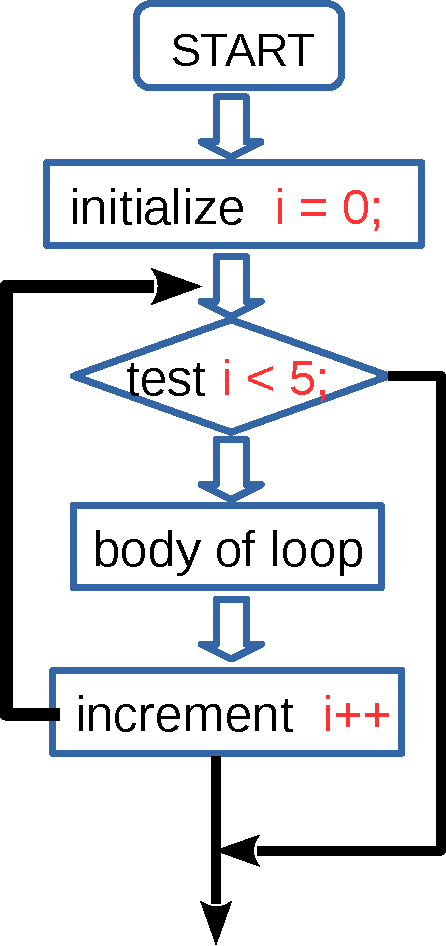
\includegraphics[width=0.20\linewidth]{figs/for.pdf}
\end{figure}
\end{frame}

\begin{frame}[fragile]{for loop (2)}
\begin{itemize}
	\item {Consider a program printing the numbers 1 to 10:}
\end{itemize}
\begin{lstlisting}[numbers=none, language=c]
int i;
for (i = 1; i <= 10; ++i)
{
    printf("%d\n", i);
}
\end{lstlisting}
\begin{itemize}
	\item {\textcolor{red}{i} starts from \textcolor{green}{1}}
	\item {Check if \textcolor{red}{i} is less than or equal to \textcolor{green}{10}}
	\item {Go into the loop if it is true (non-zeor)}
	\item {Increment \textcolor{red}{i}, e.g., i++ or i+=2}
\end{itemize}
\end{frame}

\begin{frame}[fragile]{break}
\begin{itemize}
	\item {Similar as \textcolor{blue}{switch}-\textcolor{blue}{case}}
	\item {\textcolor{blue}{break} can be used inside a loop}
	\item {Jumping out from the loop as soon as it is called}
\end{itemize}
\begin{lstlisting}[numbers=none, language=c,linewidth=0.7\linewidth]
int i, s = 0;
for (i = 1; i <= 10; ++i)
{
    s += 2*i;
    if(i%4 == 0)
    break;
}
printf("s=%d\n", s);
\end{lstlisting}
\end{frame}

\begin{frame}[fragile]{continue}
\begin{itemize}
	\item {Different from \textcolor{blue}{break}}
	\item {\textcolor{blue}{continue} can be \textcolor{red}{ONLY} used inside a loop}
	\item {Ingore statements followed, go to next round of loop}
\end{itemize}
\begin{columns}
\begin{column}{0.48\linewidth}
\begin{lstlisting}
int i, s = 0;
for (i = 1; i <= 10; ++i)
{
    s += 2*i;
    if(i%4 == 0)
    break;
}
printf("s=%d\n", s);
\end{lstlisting}
\end{column}
\begin{column}{0.02\linewidth}
\end{column}
\begin{column}{0.45\linewidth}
\begin{lstlisting}
int i, s = 0;
for (i = 1; i <= 10; ++i)
{
    s += 2*i;
    if(i%4 == 0)
    continue;
}
printf("s=%d\n", s);
\end{lstlisting}
\end{column}
\end{columns}
\end{frame}

\subsection{Examples of Loops}
\begin{frame}<beamer>
    \frametitle{Outline}
    \tableofcontents[currentsection,currentsubsection]
\end{frame}

\begin{frame}[fragile]{Example 2 (1)}
\begin{itemize}
	\item {Given following series of fraction}
	\item {$\frac{2}{1}$, $\frac{3}{2}$, $\frac{5}{3}$, $\frac{8}{5}$, $\frac{13}{8}$, $\frac{21}{13}$,$\cdots$}
	\item {Work out the sum of first \textit{20} terms}
\end{itemize}

\begin{center}
	\Large{3 minutes to think about this problem ...}
\end{center}
\end{frame}

\begin{frame}[fragile]{Example 2 (2)}
\begin{itemize}
	\item {Given following series of fraction}
	\item {$\frac{2}{1}$, $\frac{3}{2}$, $\frac{5}{3}$, $\frac{8}{5}$, $\frac{13}{8}$, $\frac{21}{13}$,$\cdots$}
	\item {Work out the sum of first \textit{20} terms}
\end{itemize}

\begin{itemize}
	\item {We observe that numerator is the sum of the numerators of last two}
	\item {The denominator is the sum of the denominators of last two}
	\item {We have following things first}
\end{itemize}
\begin{lstlisting}[linewidth=0.7\linewidth]
float n1 = 2, n2 = 3;
int d1 = 1, d2 = 2;
for (i = ?; i <= 20; ++i)
{
   ....
}
\end{lstlisting}
\end{frame}

\begin{frame}[fragile]{Example 2 (3)}
\begin{itemize}
	\item {Given following series of fraction}
	\item {$\frac{2}{1}$, $\frac{3}{2}$, $\frac{5}{3}$, $\frac{8}{5}$, $\frac{13}{8}$, $\frac{21}{13}$,$\cdots$}
	\item {Work out the sum of first \textit{20} terms}
\end{itemize}

\begin{itemize}
	\item {We need the variable to keep the result}
	\item {We need an iterator}
\end{itemize}
\begin{lstlisting}[linewidth=0.7\linewidth]
float n1 = 2, n2 = 3;
int d1 = 1, d2 = 2, i = 0;
float s = n1/d1 + n2/d2;
for (i = ?; i <= 20; ++i)
{
   ....
}
printf("s=%f\n", s);
\end{lstlisting}
\end{frame}

\begin{frame}[fragile]{Example 2 (4)}
\begin{itemize}
	\item {Given following series of fraction}
	\item {$\frac{2}{1}$, $\frac{3}{2}$, $\frac{5}{3}$, $\frac{8}{5}$, $\frac{13}{8}$, $\frac{21}{13}$,$\cdots$}
	\item {Work out the sum of first \textit{20} terms}
\end{itemize}

\begin{itemize}
	\item {We need an iterator, start from where??}
	\item {How to work out \textit{n1} and \textit{d1}}
\end{itemize}
\begin{lstlisting}[linewidth=0.7\linewidth]
float n1 = 2, n2 = 3;
int d1 = 1, d2 = 2, i = 0;
float s = n1/d1 + n2/d2;
for(i = ?; i <= 20; ++i)
{
   n1 = ?;
   d1 = ?;
   s += n1/d1;
}
printf("s=%f\n", s);
\end{lstlisting}
\end{frame}

\begin{frame}[fragile]{Example 2 (5)}
\begin{itemize}
	\item {Given following series of fraction}
	\item {$\frac{2}{1}$, $\frac{3}{2}$, $\frac{5}{3}$, $\frac{8}{5}$, $\frac{13}{8}$, $\frac{21}{13}$,$\cdots$}
	\item {Work out the sum of first \textit{20} terms}
\end{itemize}

\begin{itemize}
	\item {The full story}
\end{itemize}
\vspace{-0.1in}
\begin{columns}
\begin{column}{0.56\linewidth}
\begin{lstlisting}[linewidth=0.85\linewidth]
#include <stdio.h>
int main()
{
  float n1 = 2, n2 = 3;
  int d1 = 1, d2 = 2, i = 0;
  float s = n1/d1 + n2/d2;
  for(i = 3; i <= 20; ++i)
  {
     n2 = n1 + n2;
     d2 = d1 + d2;
     s += n2/d2;
     n1 = n2 - n1;
     d1 = d2 - d1;
  }
}
\end{lstlisting}
\end{column}
\begin{column}{0.4\linewidth}
\begin{lstlisting}[firstnumber=15]
  printf("s=%f\n", s);
  return 0;
}
\end{lstlisting}
\end{column}
\end{columns}
\end{frame}


\begin{frame}[fragile]{Example 3 (1)}
\begin{itemize}
	\item {Output following figure}
\end{itemize}
\begin{center}
\Large{
    * \\
   ***\\
  *****\\
 *******\\
  *****\\
   ***\\
    *
}
\end{center}
\end{frame}

\begin{frame}[fragile]{Example 3 (2)}
\begin{itemize}
	\item {On the 1st line, we print 3 blanks and 1 star}
    \item {On the 2nd line, we print 2 blanks and 3 stars}
    \item {On the 3rd line, we print 1 blanks and 5 stars}
    \item {On the 4th line, we print 0 blank  and 7 stars}
    \item {Do the following in reverse...}
\end{itemize}
\begin{itemize}
	\item {There should be a loop controls of printing blanks of one line}
    \item {There should be a loop controls of printing stars of one line}
    \item {There should be a loop controls of printing all the lines}
    \item {How to organize them??}
\end{itemize}

\end{frame}

\begin{frame}[fragile]{Example 3 (3)}
\begin{itemize}
	\item {There should be a loop controls of printing blanks of one line}
    \item {There should be a loop controls of printing stars of one line}
    \item {There should be a loop controls of printing all the lines}
    \item {How to organize them??}
\end{itemize}
\begin{enumerate}
	\item {Loop print all lines}
	\item {~~Loop print blank(s)}
	\item {~~Loop print star(s)}
	\item {End-Loop}
\end{enumerate}

\end{frame}

\begin{frame}[fragile]{Example 3 (4)}
\begin{enumerate}
	\item {Loop print all lines}
	\item {~~Loop print blank(s)}
	\item {~~Loop print star(s)}
	\item {End-Loop}
\end{enumerate}
\begin{enumerate}
	\item {We need a bound for the number of stars}
	\item {We need a bound for the number of blanks}
\end{enumerate}
\begin{lstlisting}
 int n = 7, i = 0, j = 0;
 int ns = 1, nb = n-1;
 for(i = 0; i < n; i++)
 {
    ...
 }
\end{lstlisting}
\end{frame}

\begin{frame}[fragile]{Example 3 (5)}
\begin{enumerate}
	\item {Print things to the bounds}
\end{enumerate}
\vspace{-0.1in}
\begin{columns}
\begin{column}{0.49\linewidth}
\begin{lstlisting}[numbers=none]
 int n = 5, i = 0, j = 0;
 int ns = 1, nb = n-1;
 for(i = 0; i < n; i++)
 {
    for(j = 0; j < nb; j++)
    {
       printf(" ");
    }
    for(j = 0; j < ns; j++)
    {
       printf("*");
    }
    ns += 2;
    nb--;
    printf("\n");
 }
\end{lstlisting}
\end{column}
\begin{column}{0.49\linewidth}
\begin{lstlisting}[numbers=none]
 nb += 2; //<--why?
 ns -= 4; //<--why?
 for(i = 0; i < n; i++)
 {
    for(j = 0; j < nb; j++)
    {
       printf(" ");
    }
    for(j = 0; j < ns; j++)
    {
       printf("*");
    }
    ns -= 2;
    nb++;
    printf("\n");
 }
\end{lstlisting}
\end{column}
\end{columns}
\end{frame}


\begin{frame}[fragile]{Example 4 (1): solving by exhaustive search}
\begin{itemize}
   \item {30 people dine together, 50 cents are paid}
   \item {It takes 3 cents for a gentleman}
   \item {It takes 2 cents for a lady}
   \item {It takes 1 cent for a child}
   \item {How many gentlemen, ladies and children are there}
\end{itemize}
\begin{equation}
\left \{ \begin{array}{l}
  3*x+2*y+z=50 \\
  x+y+z=30
\end{array} \right.  \nonumber
\end{equation}
\begin{itemize}
	\item {We are actually trying to solve linear equations}
	\item {Notice that only integer solutions are valid}
\end{itemize}
\end{frame}

\begin{frame}[fragile]{Example 4 (2): solving by exhaustive search}
\begin{itemize}
   \item {Solution is, we enumerate all possible solution}
   \item {To see whether they satisfy all the equations}
\end{itemize}
\begin{equation}
\left \{ \begin{array}{l}
  3*x+2*y+z=50 \\
  x+y+z=30
\end{array} \right.  \nonumber
\end{equation}
\begin{itemize}
	\item {Enumerate \textit{x} from 1 to 30}
	\item {Enumerate \textit{y} from 1 to 30}
	\item {Enumerate \textit{z} from 1 to 30}
	\item {Now let's do it!}
\end{itemize}
\end{frame}

\begin{frame}[fragile]{Example 4 (3): solving by exhaustive search}
\begin{itemize}
	\item {Enumerate \textit{x} from 1 to 30}
	\item {Enumerate \textit{y} from 1 to 30}
	\item {Enumerate \textit{z} from 1 to 30}
\end{itemize}
\begin{equation}
\left \{ \begin{array}{l}
  3*x+2*y+z=50 \\
  x+y+z=30
\end{array} \right.  \nonumber
\end{equation}
\begin{lstlisting}[numbers=none]
for(x = 1; x <= 30; x++)
{
   for(y = 1; y <= 30; y++)
   {
       for(z = 1; z <= 30; z++)
       {
         ....
       }
   }   
}
\end{lstlisting}
\end{frame}

\begin{frame}[fragile]{Example 4 (4): solving by exhaustive search}
\vspace{-0.15in}
\begin{lstlisting}[]
#include <stdio.h>
int main()
{
  int x = 0, y = 0, z = 0, c1 = 0, c2 = 0;
  for(x = 1; x <= 30; x++)
  { for(y = 1; y <= 30; y++)
     { for(z = 1; z <= 30; z++)
       {
          c1 = 3*x+2*y+z;
          c2 = x+y+z;
          if(c1 == 50 && c2 == 30)
          {
              printf("x = %d, y = %d, z = %d\n", x,y,z);
          }
       }//for(z)
   }//for(y)
  }//for(x)
 }
\end{lstlisting}
\end{frame}

\begin{frame}[fragile]{Example 4 (5): solving by exhaustive search}
\vspace{-0.15in}
\begin{lstlisting}[]
#include <stdio.h>
int main()
{
  int x = 0, y = 0, z = 0, c1 = 0, c2 = 0;
  for(x = 1; x < 17; x++) //<-- why??
  { for(y = 1; y <= 25; y++) //<-- why??
     { for(z = 1; z <= 30; z++)
       {
          c1 = 3*x+2*y+z;
          c2 = x+y+z;
          if(c1 == 50 && c2 == 30)
          {
              printf("x = %d, y = %d, z = %d\n", x,y,z);
          }
       }//for(z)
   }//for(y)
  }//for(x)
 }
\end{lstlisting}
\end{frame}


\section{Miscellaneous}
\label{sec:misc}
\begin{frame}<beamer>
    \frametitle{Outline}
    \tableofcontents[currentsection]
\end{frame}

\begin{frame}[fragile]{Try to avoid following case}
\begin{itemize}
	\item {Be careful, this}
\end{itemize}

\begin{lstlisting}
while (1 > 0)
	printf("Did you miss me?\n");
\end{lstlisting}
\begin{itemize}
	\item {Runs till the end of all days}
    \item {$\infty$ loops are common mistakes, and you will experience many of them}
	\item {Check for conditions that are always true}
	\item {By the way,}
\end{itemize}
\begin{center}
 \Huge {Do not be evil!}
\end{center}
\end{frame}

\begin{frame}[fragile]{Valid variants of for-loop (1)}
\begin{itemize}
	\item {The arguments for the \textcolor{blue}{for} loop are optional}
	\item {If you already have defined your iterating variable}
\end{itemize}
	\begin{lstlisting}[numbers=none]
int i = 1;
for (; i <= 10; ++i)
	printf("%d\n", i);
\end{lstlisting}

\begin{itemize}
	\item {Or if you have the iteration statement in your loop body}
\end{itemize}
	\begin{lstlisting}[numbers=none, language=c]
for (i = 1; i <= 10;)
	printf("%d\n", ++i);	/* seems more like a while loop */
\end{lstlisting}
\end{frame}

\begin{frame}[fragile]{Valid variants of for-loop (2)}
\begin{itemize}
	\item {If you're not passing anything, it runs \textbf{for}ever}
\end{itemize}
	\begin{lstlisting}[numbers=none]
for (;;)
	printf("I'm still here\n");
\end{lstlisting}
Note: the semicolons are still there.
\end{frame}



